\chapter{INVERSÃO DO MODELO DE VELOCIDADES}
\label{cap8:velocidades}

Propomos a seguinte metodologia para a inversão do modelo de velocidades e cumprimento do objetivo da tese:
Utilizar a simulação de resposta de difrações com a aproximação de tempo de trânsito ERC (Equação \ref{eq:2.3}) ou
a aproximação de tempo de trânsito do SRC não hiperbólico (Equação \ref{eq:2.4}), 
com aplicação da condição SDC ($R_N=R_{NIP}$),
para simular as difrações \cite{diffractions}.

O conceito de determinação da velocidade através da simulação de resposta de difração
consiste dos seguintes passos \cite{diffractions}:

\begin{enumerate}
 \item Determinação da velocidade NMO: Isto pode ser feito em cascata nos pontos da
seção empilhada, camada por camada otimizando a velocidade uma camada por vez.
\item Determinação dos slopes de reflexão de afastamento nulo no cubo de dados empilhados: 
Este passo não será necessário na nova metodologia.
\item Transformação dos traços zero offset selecionados em respostas de pontos difratores em CDP's
selecionados.
\item Aplicação da migração em profundidade pós empilhamento com análise de velocidades
em looping.
\end{enumerate}

A partir da seção empilhada ERC transformamos cada par $m_0, t_0$ sobre um refletor em uma resposta simulada de
uma fonte pontual (Ponto difrator) na forma de hipérboles de difração. Escolhido um par $m_0, t_0$, ele terá um par
de parâmetros $R_{NIP}, \beta_0$ que possibilitam traçar uma hipérbole de difração a partir da aproximação do SRC
não hiperbólico utilizando a condição SDC ($R_N=R_{NIP}$).

Espalhando o valor de amplitude do ponto escolhido na seção empilhada $A(m_0,t_0)$ sobre a hipérbole de difração
previamente calculada, teremos a resposta simulada de uma difração \cite{diffractions}. A inversão do modelo de velocidades
se torna a busca pelas velocidades de migração que melhor focalizam as hipérboles de difração simuladas.

Depois realizaremos a análise de velocidades automatizada no domínio pós empilhado e o imageamento de alta resolução
para heterogeneidades de pequena escala produzindo imagens migradas no tempo com as hipérboles de difração
focalizadas. Este processo contará com a análise automatizada de focalização para a detecção das
velocidades de migração ótimas para imageamento das hipérboles de difração simuladas \cite{sep_dif}.

A migração será realizada a partir de um algoritmo de continuação de velocidades \cite{fomel2003a}, um método que performa
a análise de velocidade de migração em tempo continuando imagens sísmicas na velocidade, também chamado de
``ondas imagem'' \cite{hubral1996}. A teoria da continuação de velocidades mostra ser possível realizar a migração no tempo
com um conjunto de diferentes velocidades fazendo pequenos incrementos na velocidade diretamente no domínio da imagem.
Implementaremos através de um algoritmo baseado na tranformada rápida de Fourier \cite{bfomel2003}.

Aplicaremos uma medida de focalização local para obter os painéis de velocidade de migração para cada ponto no domínio da
imagem. E realizaremos a análise de velocidades automatizada, com a principal diferença de que a informação sobre a velocidade
será obtida da análise da medida de focalização das difrações ao invés da coerência \cite{sep_dif}.
Os resultados obtidos são as velocidades de migração que melhor focalizam as hipérboles da seção simulada e tangente as hipérboles
aparecerá a imagem do refletor.

\begin{figure}[htb]
\caption{Fluxograma do algoritmo de inversão do modelo de velocidades.}
\begin{center}
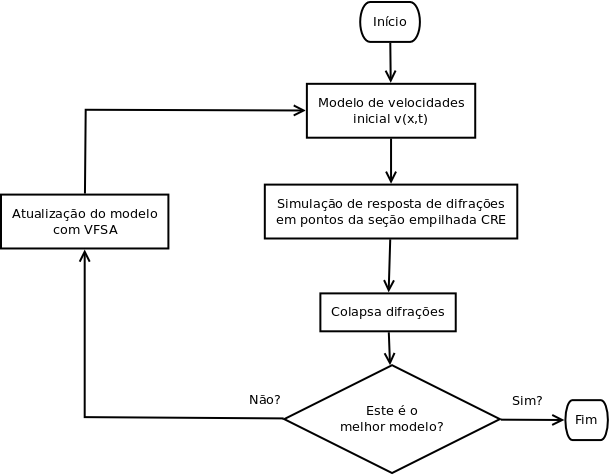
\includegraphics[scale=0.30]{images/fluxoVel.png}
\vspace{-0.3cm}
\end{center}
\begin{center}
 Fonte: Do Autor.
\end{center}
\label{fig:8.1}
\end{figure}